\chapter{Design and Implementation}
As introduced in the background analysis, current matching learning approaches to graph matching tend to generate node or graph-level representations with techniques such as graph neural network and DeepWalk and then matching the similarity of the representations. Though some have achieved remarkable accuracy rate, I believe these researches focus too much on matching the node attributes and do not emphasize enough on the structure of the graph.(problems with these approaches should be discussed before) This work proposes a model which takes both attributes and structure into account.

\section{Smart Design}
\label{sec:des-hotpath}
The target problem has two connected large graphs G and G', where the model needs to find top-k matching connected subgraphs in G' for any given connected subgraph in G. G and G' have node features. (add examples and matching examples here)

The proposed model(come up with a name later) has two main parts, which aims to matching the features and structures of graphs respectively. To study the graph features, the first part uses graph neural networks coupled with multilayer perceptrons to generate embeddings of nodes. The second part of the model is inspired from well-established approaches in natural language processing(NLP). It introduces the novel idea of treating graphs as sequences of nodes and processing them with a Long Short-Term Memory(LSTM) to study the correlation between the nodes. 

\subsection{Dataset}
The problem takes the whole graphs G and G' as inputs, but the model trains on pairs of their constituent subgraphs. For the first step, generated training data is used. The generation process is recurrent with two stages.

\subsubsection{Pair Generation}
The first stage is generating two random matching connected graphs g and g'. This is achieved by generating g first and construct a matching one g' based on certain criteria. In this experiment, I use g containing 5 nodes, each with a unique node id and one attribute "color". The domain of "color" is "red", "blue" and "yellow". The density of g is 0.5. g' has the same number of nodes and node ids as g. The criteria determining that g' is matched to g is based on two parameters: w$_n$, the significance of node attributes and w$_s$, the significance of structure. Both parameters are constants between 0 and 1.

w$_n$ denotes the probability that attribute values are the same for nodes with the same id. If w$_n$ is 1, nodes with the same id in both graphs have the same attributes values and if it is 0, the node attributes in g' are randomly selected from the domain excluding the value taken by the corresponding node in g.(example).

w$_s$ is the probability that an edge in g is kept in g' and g' containing an edge which does not appear in g. If it is 1, g and g' have the exact same edges and if it is 0, both graphs do not contain the same edges unless they are necessary to keep g' connected. (example)

During the training process, Three sets of values for w$_n$ and w$_s$ are used to evaluate the performance: 0 0, 0.5 0.5 and 1 1(remove this note: currently using 0.5,0.5).
\subsubsection{Graph Aggregation}
The problem inputs are large connected graphs G and G'. Therefore, each time when generating a new pair of subgraphs g and g', an existing node with is selected from G and G' with the same node id and reused in the new pair. 
\newline
\newline
In this setup, 5 pairs of matching subgraphs of 5 nodes are generated, the resultant G and G' both have 21 nodes. Therefore, there are five instances of training data. The generated graphs are then encoded using one-hot encoding, resulting in each graph represented by a 21*3 matrix. (optionly, add connectivity as additional attributes)

\subsection{Node Embedding}
\subsubsection{Graph Neural Network(GNN)}
(introduce GNN, add image, explanation, citation, emphasize on its ability to embed features and capture neighbourhood information)

\subsubsection{GNN in (this model)}
The power of GNN makes it a natural choice for generating node embedding for (this model). 

\begin{figure}[H]
  \centering
  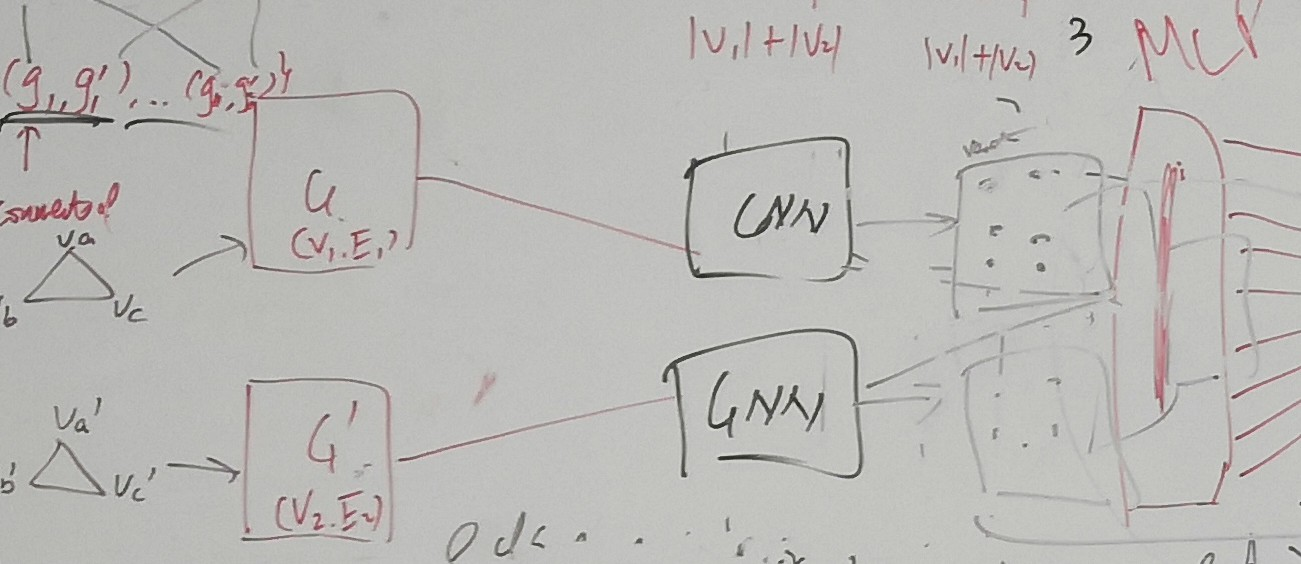
\includegraphics[width=0.80\textwidth]{embedding.jpg}
  \caption{to be changed into a better one with clear label}
\end{figure}

Figure 3.1 shows the structure of the embedding section. The inputs are the pairs of subgraphs each encoded into a 5*3 matrix, as well as their adjacency matrix. The model contains one 2-hop GNN with 3-dimensional messages for each input graph followed by a single fully connected layer(later replace with Wasserstein layer or add another section to compare with Wasserstein). For each node in the input, the output embedding is in R$^{5}$. Aggregating the node representations gives two 5*5 matrices for each pair of inputs.

\subsubsection{Embedding Loss}
The loss for the embedding process is the Enclidean distance between the output matrices, denoted as L1. (Add formula) Ideally, if the two input graphs are the same, the output should be the same, so the loss should be 0. 

\subsection{Structure Matching}
Though GNN is capable of capturing neighbourhood information by message passing hence capture some degree of structural information, this kind of information is not reflected if matching is done by looking for the node with the closest embedding in the other graph. Hence, it is very likely that these generated nodes are not connected in the original graph. Furthermore, if the training subgraphs get large, message passing within larger neighbourhoods may be necessary. The computational cost of extra layers of GNN increases exponentially for dense graphs.

Therefore, the second part of (the model) aims to capture structure information of graphs. Inspired by approaches used in natural language processing(included in background analysis), if graphs can be treated as sequential data(structurally) similarly, the rich resort of NLP methods may be utilized for this problem as well. Here, the nodes are sequenced in the order of ascending node id. However, it may not be accurate if nodes after have a correspondence with previous ones, therefore, the reverse direction is also considered. This part of (the model) contains a LSTM and a fully-connected layer at the end.

\subsubsection{LSTM}
(explain LSTM, graph, or include in background analysis)

\subsubsection{LSTM in (this model)}
The output of the embedding section for each pair of matching subgraphs are two matrices of size 5*5, m and m'. Only m which represents the embedding of g, the subgraph of G is fed as input since the output is compared against m' to compute the loss. (Or use both and find the matching ones for both, double the training data) (This model) uses a bi-directional LSTM with two layers to increase its generalization power. Each layer has 4 hidden units so that it is smaller than the input size in order to restrict the functionality of each layer and reduce the total number of hidden neurons. The output dimension is 5, the same as input.

\subsubsection{Matching Loss}
For each output o produced, the node with the closest embedding in G' is found by comparing the euclidean distance between their embedding vectors and o. The embedding of the five nodes found are then aggregated into a matrix m" and the model computes the Euclidean distance L2 between m" and m' as the matching loss(add formula). 

The total loss of the model is L1 + $\lambda$L2, where $\lambda$ is a constant between 0 and 1.

\section{Section summary}

(To be updated as I progress)